% ===========================================================================
%  Research Poster (A0, portrait, tikzposter)
%  A Systematic Comparison of Large Language Models and Small Language Models
%  in Standalone, Hybrid, and Multi-Agent Architectures
%  Department of Computer Engineering, Izmir Institute of Technology
%
%  Build:  pdflatex main.tex   (from this directory)
%  Needs:  tikzposter, pgfplots, qrcode  (tlmgr --usermode install ...)
% ===========================================================================
\documentclass[25pt, a0paper, portrait, margin=12mm, innermargin=9mm,
               blockverticalspace=2mm, colspace=10mm, subcolspace=8mm]{tikzposter}

\usepackage[T1]{fontenc}
\usepackage[utf8]{inputenc}
\usepackage{lmodern}
\usepackage{amsmath}
\usepackage{amssymb}
\usepackage{graphicx}
\usepackage{booktabs}
\usepackage{tabularx}
\usepackage{array}
\usepackage{qrcode}
\usepackage{pgfplots}
\pgfplotsset{compat=1.18}
\usetikzlibrary{positioning, arrows.meta, shapes.geometric}

\graphicspath{{figures/}}
\renewcommand{\familydefault}{\sfdefault}

% --- Color scheme (IZTECH claret + slate) ----------------------------------
\definecolor{iyteClaret}{HTML}{8A1538}
\definecolor{iyteDark}{HTML}{2B2D42}
\definecolor{accentTeal}{HTML}{0F7173}
\definecolor{accentGold}{HTML}{C8963E}
\definecolor{lightBg}{HTML}{F4F1ED}

\definecolorstyle{IZTECHStyle}{
  \colorlet{colorOne}{iyteClaret}
  \colorlet{colorTwo}{iyteDark}
  \colorlet{colorThree}{accentTeal}
}{
  % Background
  \colorlet{backgroundcolor}{white}
  \colorlet{framecolor}{white}
  % Title
  \colorlet{titlefgcolor}{white}
  \colorlet{titlebgcolor}{iyteClaret}
  % Blocks
  \colorlet{blocktitlebgcolor}{iyteClaret}
  \colorlet{blocktitlefgcolor}{white}
  \colorlet{blockbodybgcolor}{white}
  \colorlet{blockbodyfgcolor}{iyteDark}
  % Inner blocks
  \colorlet{innerblocktitlebgcolor}{lightBg}
  \colorlet{innerblocktitlefgcolor}{iyteDark}
  \colorlet{innerblockbodybgcolor}{lightBg}
  \colorlet{innerblockbodyfgcolor}{iyteDark}
  % Notes
  \colorlet{notefgcolor}{iyteDark}
  \colorlet{notebgcolor}{lightBg}
  \colorlet{noteframecolor}{iyteClaret}
}

\usetheme{Default}
\usecolorstyle{IZTECHStyle}
\useblockstyle{Minimal}
\usetitlestyle{Filled}

% Hide the tikzposter watermark in the bottom-right corner
\tikzposterlatexaffectionproofoff

% --- Stat card helper: number, caption line 1, caption line 2, color --------
\newcommand{\statcard}[4]{%
  \begin{tikzpicture}
    \node[rectangle, rounded corners=8pt, fill=lightBg, draw=#4, line width=2.5pt,
          text width=0.26\linewidth, minimum height=4.2cm, align=center, inner sep=8pt]
      {{\fontsize{52}{56}\selectfont\bfseries\color{#4} #1}\\[6pt]
       {\normalsize\color{iyteDark} #2}\\
       {\normalsize\color{iyteDark} #3}};
  \end{tikzpicture}%
}

% --- Title content -----------------------------------------------------------
\title{\parbox{0.94\linewidth}{\centering\fontsize{72}{82}\selectfont\bfseries
A Systematic Comparison of Large and Small Language Models\\
in Standalone, Hybrid, and Multi-Agent Architectures}}
\author{\large Do\u{g}ukan Top\c{c}u \quad\textbullet\quad Abdulbaki \c{C}eltik
\quad\textbullet\quad Berkhan Karg\i l\i{} \quad\textbullet\quad Meri\c{c} Kelemeden\\[8pt]
\normalsize Advisors: Dr.\ H\"useyin \"Unl\"u \quad\textbullet\quad Prof.\ Dr.\ Onur Demir\"ors}
\institute{\normalsize Department of Computer Engineering, \.{I}zmir Institute of Technology, \.{I}zmir, T\"urkiye --- June 2026}

\makeatletter
\settitle{%
  \begin{minipage}[c]{0.12\linewidth}
    \centering
    
\includegraphics[width=0.85\linewidth]{iyte_logo.png}
  \end{minipage}%
  \begin{minipage}[c]{0.86\linewidth}
    \centering
    {\color{titlefgcolor}\@title\par}
    \vspace{0.55cm}
    {\color{titlefgcolor}\@author\par}
    \vspace{0.35cm}
    {\color{titlefgcolor}\@institute\par}
  \end{minipage}%
}
\makeatother

\begin{document}
\maketitle[width=\linewidth]

\begin{columns}

% ============================ LEFT COLUMN ===================================
\column{0.34}

\block{1\,\textbar\, Motivation, RQs \& Review Method}{
\textbf{Problem.} LLMs deliver state-of-the-art reasoning, but often at substantial
\textbf{latency, monetary cost, and energy overhead}. SLMs offer a cheaper and more
data-sovereign alternative, yet still trail frontier LLMs on broad reasoning tasks.
\textbf{Literature gap.} Our companion systematic review of \textbf{54 collaborative
SLM--LLM studies} shows a reporting asymmetry: hybrid and multi-agent designs are increasing,
but \textbf{cost and energy are rarely treated as first-class outcomes} alongside accuracy.

\vspace{6pt}
\textbf{Objective.} We ask a systems-design question: \emph{which orchestration architecture
provides the best capability--efficiency trade-off under real deployment conditions?}
To answer this, we built a \textbf{measurement-first evaluation platform} and introduce
\textbf{EATS} to jointly rank accuracy, latency, cost, and energy.

\vspace{8pt}
\innerblock{Research Questions}{%
\begin{itemize}
  \item \textbf{RQ1 Performance:} how do collaborative SLM/LLM systems compare with monolithic LLMs on reasoning and classification tasks?
  \item \textbf{RQ2 Efficiency:} how do hybrid and multi-agent designs affect inference cost, latency, and energy?
  \item \textbf{RQ3 Orchestration:} which routing and division-of-labor mechanisms are used across architectures?
  \item \textbf{RQ4 Domain suitability:} where do collaborative systems match LLM baselines, and where do they fail?
\end{itemize}}

\vspace{6pt}
\begin{center}
\textbf{Systematic Review Method}\\[6pt]
\includegraphics[width=0.82\linewidth]{prisma_flowchart.pdf}
\end{center}
}

\block{2\,\textbar\, Measurement-First Platform}{
Every architecture consumes the same \texttt{Query} and returns the same \texttt{Response}
carrying \textbf{accuracy, latency, tokens, cost, energy, and CO$_2$} per query. The
architecture layer is the \emph{only} interchangeable component.

\vspace{6pt}
\centering
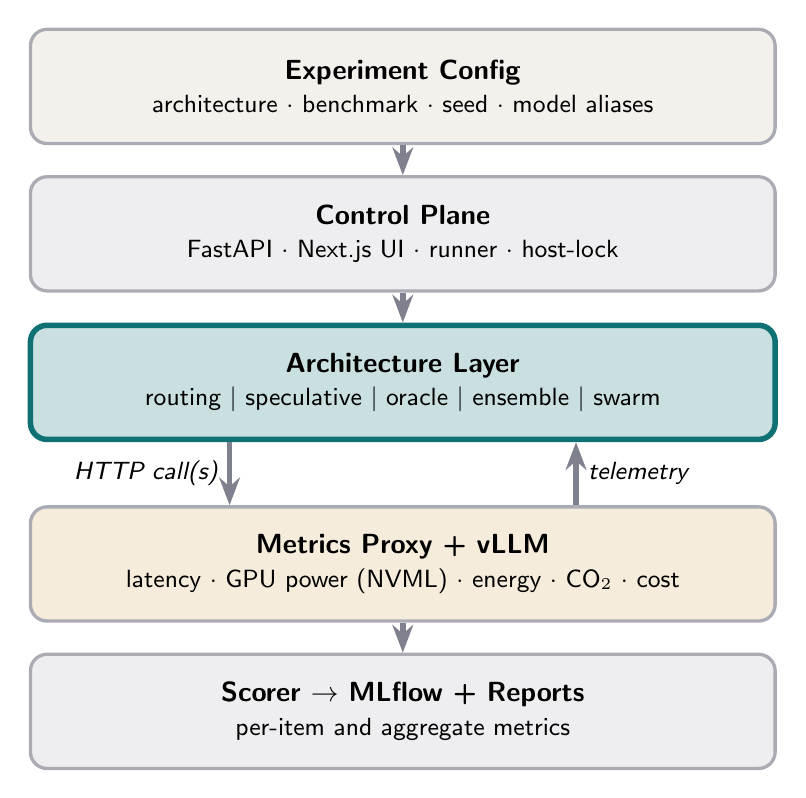
\begin{tikzpicture}[
  node distance=0.38cm,
  box/.style={rectangle, rounded corners=6pt, draw=iyteDark!40, line width=1.2pt,
              minimum width=0.78\linewidth, minimum height=1.45cm, align=center,
              inner sep=8pt, font=\normalsize},
  arrow/.style={-{Stealth[length=10pt]}, line width=2pt, draw=iyteDark!60}
]
\node[box, fill=lightBg] (config) {\textbf{Experiment Config}\\
  {\small architecture $\cdot$ benchmark $\cdot$ seed $\cdot$ model aliases}};
\node[box, fill=iyteDark!8, below=of config] (cp) {\textbf{Control Plane}\\
  {\small FastAPI $\cdot$ Next.js UI $\cdot$ runner $\cdot$ host-lock}};
\node[box, fill=accentTeal!22, draw=accentTeal, line width=2pt, below=of cp] (arch)
  {\textbf{Architecture Layer}\\
  {\small routing $|$ speculative $|$ oracle $|$ ensemble $|$ swarm}};
\node[box, fill=accentGold!18, below=0.8cm of arch] (proxy) {\textbf{Metrics Proxy + vLLM}\\
  {\small latency $\cdot$ GPU power (NVML) $\cdot$ energy $\cdot$ CO$_2$ $\cdot$ cost}};
\node[box, fill=iyteDark!8, below=of proxy] (out) {\textbf{Scorer $\rightarrow$ MLflow + Reports}\\
  {\small per-item and aggregate metrics}};
\draw[arrow] (config) -- (cp);
\draw[arrow] (cp) -- (arch);
\draw[arrow] ([xshift=-2.2cm]arch.south) -- node[left, font=\small\itshape]{HTTP call(s)} ([xshift=-2.2cm]proxy.north);
\draw[arrow] ([xshift=2.2cm]proxy.north) -- node[right, font=\small\itshape]{telemetry} ([xshift=2.2cm]arch.south);
\draw[arrow] (proxy) -- (out);
\end{tikzpicture}

\vspace{4pt}
\raggedright
\textbf{GPU inference plane} (open-weight models, vLLM serving):
\begin{center}
\footnotesize
\begin{tabular}{@{} l l l l @{}}
\toprule
\textbf{Tier} & \textbf{Host} & \textbf{VRAM} & \textbf{Models} \\
\midrule
SLM (dedicated)  & GCP L4          & 24\,GB  & Gemma\,/\,Qwen\,/\,LLaMA\,/\,Ministral, 3--4B \\
Mid (shared)     & GCP RTX PRO6000 & 96\,GB  & 20--35B dense + MoE checkpoints \\
Heavy (shared)   & Nebius H200     & 141\,GB & LLaMA\,3.3-70B, gpt-oss-120B \\
\bottomrule
\end{tabular}
\end{center}
}

\block{3\,\textbar\, EATS: Efficiency-Accuracy Trade-off Score}{
Accuracy $\alpha$ meets cost, latency, and energy ratios normalised by the
benchmark-specific standalone-LLM baseline ($\tilde{C}=C/C_0$, $\tilde{L}=L/L_0$, $\tilde{E}=E/E_0$):
\begin{align*}
  P &= 0.5\,\tilde{C} + 0.3\,\tilde{L} + 0.2\,\tilde{E},
  \qquad
  \text{EATS} = \frac{\alpha}{\alpha + P}
\end{align*}
\begin{itemize}
  \item Increasing in accuracy, decreasing in resource penalty; baseline reduces
        to $\alpha/(\alpha+1)$ --- a clean reference curve.
  \item Weights reflect deployment priorities: cost $>$ latency $>$ energy.
\end{itemize}
}

\block{4\,\textbar\, Energy, Carbon \& Cost Measurement}{
A per-host metrics proxy times each request and samples GPU power via NVIDIA NVML
(CodeCarbon preferred): the boundary sits \emph{at the inference host} --- real power
draw, not network overhead.
\begin{align*}
  E = \tfrac{P_{\text{GPU}}\,\Delta s}{3.6\times 10^{6}}\,\text{kWh},
  \quad
  \text{CO}_2 = k E,
  \quad
  C = C_{\text{API}} + r t
\end{align*}
$k=380$ gCO$_2$/kWh; GPU-tier rates \$0.75--\$6.50/h.
}

% =========================== MIDDLE COLUMN ==================================
\column{0.33}

\block{5\,\textbar\, Benchmarks \& Protocol}{
\textbf{88 experiments}, six architecture families, 100--520 samples per configuration,
temperature 0.0, fixed seeds, shared prompts and parsers.
\begin{center}
\small
\begin{tabular}{@{} l l @{}}
\toprule
\textbf{Benchmark} & \textbf{Capability dimension} \\
\midrule
MMLU          & world knowledge (57 subjects) \\
ARC-Challenge & science reasoning \\
GSM8K         & arithmetic reasoning (free-form) \\
HellaSwag     & commonsense continuation \\
TruthfulQA    & adversarial factual calibration \\
\bottomrule
\end{tabular}
\end{center}
}


\block{6\,\textbar\, Architecture Taxonomy}{
Ten architectures in three families; $\dagger$ marks novel designs contributed by this
project. Architectures marked $^{\ast}$ are implemented but not yet benchmarked.
\vspace{6pt}
\begin{center}
\small
\begin{tabular}{@{} l l l @{}}
\toprule
\textbf{Family} & \textbf{Architecture} & \textbf{Key mechanism} \\
\midrule
Standalone & Single-Model & one model, direct inference \\
           & MoE          & internal sparse expert activation \\
\midrule
Hybrid     & Routing      & confidence-based SLM$\to$LLM escalation \\
           & Speculative  & SLM drafts; LLM rewrites divergent suffix \\
           & Debate (POA)$^{\ast}$ & proponent--opponent--arbitrator roles \\
           & Active Oracle\,$\dagger$ & targeted LLM sub-queries on impasse \\
           & Blackboard\,$\dagger$$^{\ast}$ & bid-based task board; LLM sweeper \\
           & Entropy Blackboard\,$\dagger$$^{\ast}$ & uncertainty-penalised bidding \\
\midrule
Multi-SLM  & Ensemble     & majority / confidence-weighted voting \\
           & Pure Swarm\,$\dagger$ & SLM-only peers; no LLM online \\
\bottomrule
\end{tabular}
\end{center}

\vspace{12pt}
\begin{center}
\begin{minipage}{0.48\linewidth}
  \centering
  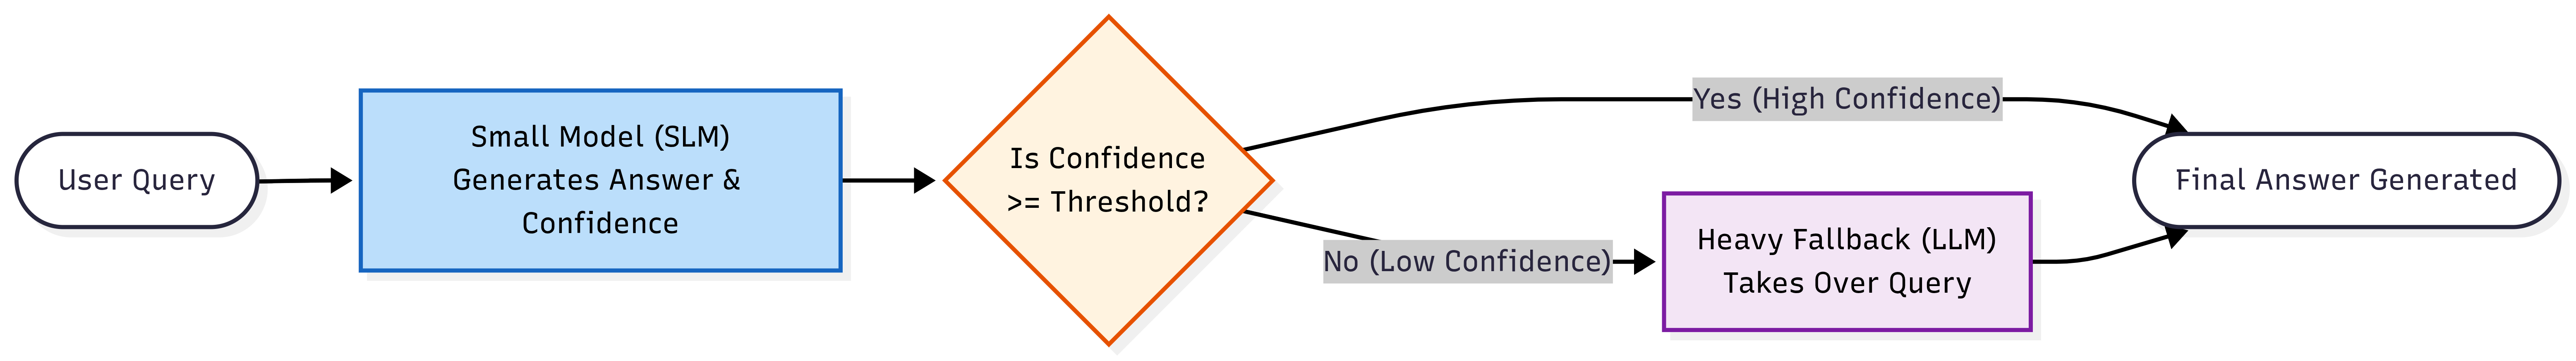
\includegraphics[width=\linewidth]{routing_simplified.png}
  {\small Routing: SLM answers first; LLM only on low confidence.}
\end{minipage}\hfill
\begin{minipage}{0.48\linewidth}
  \centering
  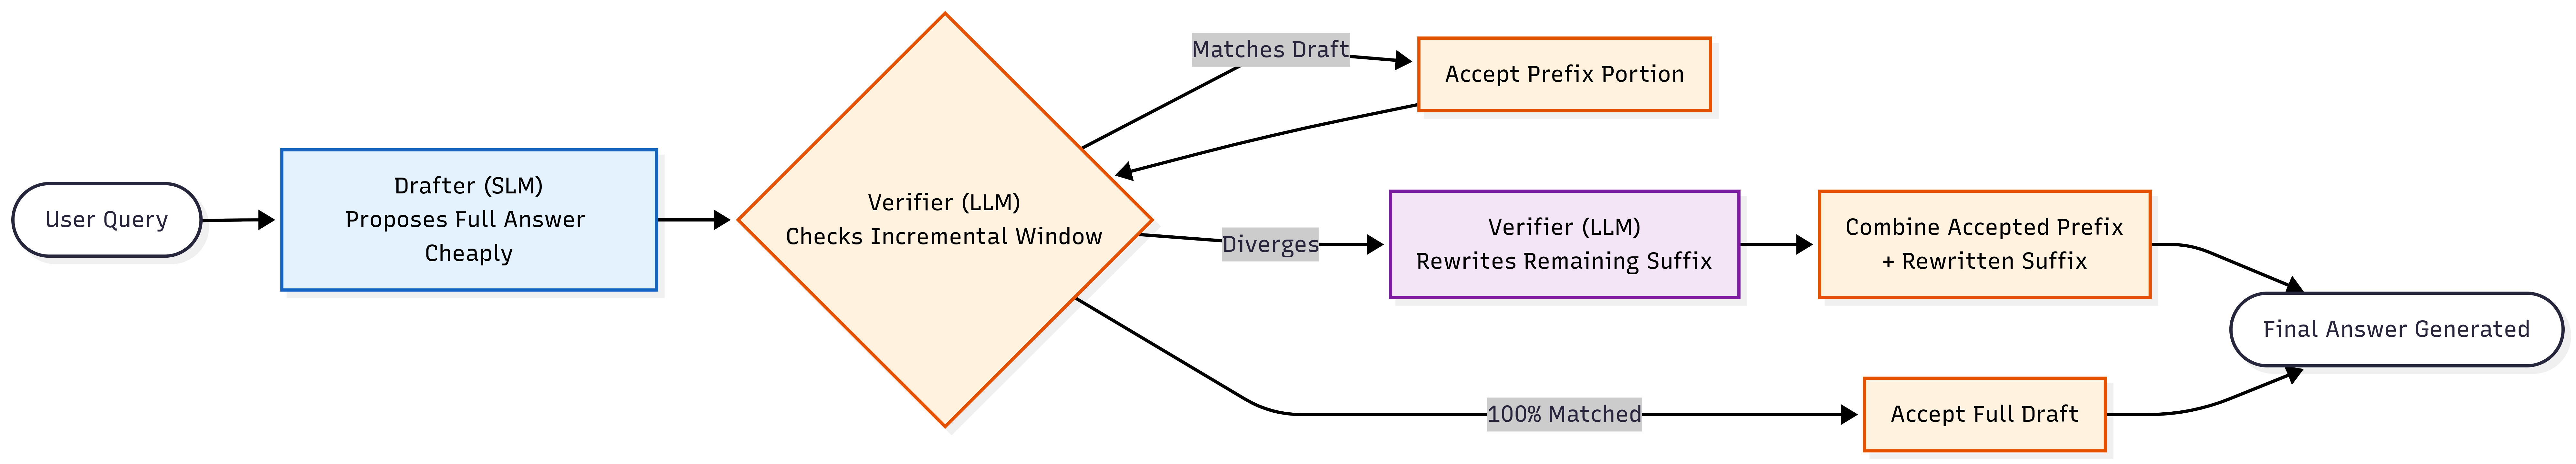
\includegraphics[width=\linewidth]{speculative_simplified.png}
  {\small Speculative: SLM drafts; LLM verifies and patches the suffix.}
\end{minipage}
\end{center}
}

\block{7\,\textbar\, EATS Frontier per Benchmark}{
Routing and speculative decoding (\texttt{gemma4-4b}$\to$\texttt{gemma4-31b}) take the top
two EATS positions on \textbf{4 of 5 benchmarks}; on GSM8K lean MoE checkpoints win because
routing escalates only 1\% of queries.
\vspace{8pt}
\begin{center}
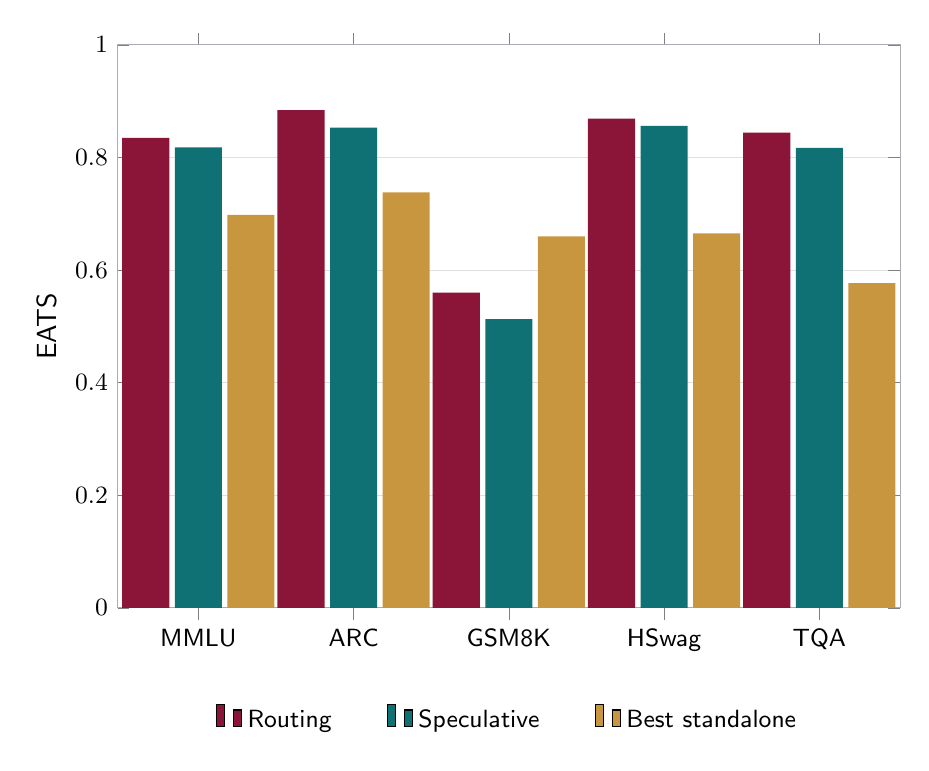
\begin{tikzpicture}
\begin{axis}[
  ybar, bar width=17pt,
  width=0.95\linewidth, height=0.72\linewidth,
  ymin=0, ymax=1.0,
  ylabel={EATS},
  symbolic x coords={MMLU, ARC, GSM8K, HSwag, TQA},
  xtick=data,
  ymajorgrids,
  grid style={iyteDark!15},
  axis line style={iyteDark!40},
  tick label style={font=\small},
  label style={font=\normalsize},
  legend style={at={(0.5,-0.16)}, anchor=north, legend columns=3, font=\small,
                draw=none, /tikz/every even column/.append style={column sep=18pt}},
  enlarge x limits=0.13,
]
\addplot[fill=iyteClaret,  draw=none] coordinates
  {(MMLU,0.835) (ARC,0.884) (GSM8K,0.560) (HSwag,0.869) (TQA,0.844)};
\addplot[fill=accentTeal,  draw=none] coordinates
  {(MMLU,0.818) (ARC,0.853) (GSM8K,0.513) (HSwag,0.856) (TQA,0.817)};
\addplot[fill=accentGold,  draw=none] coordinates
  {(MMLU,0.698) (ARC,0.738) (GSM8K,0.660) (HSwag,0.665) (TQA,0.577)};
\legend{Routing, Speculative, Best standalone}
\end{axis}
\end{tikzpicture}
\end{center}
}

\block{8\,\textbar\, Limitations}{
\begin{itemize}
  \item Pilot scale: 100--520 samples per configuration; no significance tests yet ---
        results are directional, not definitive.
  \item All routing / speculative runs use one SLM--LLM pair
        (\texttt{gemma4-4b}$\to$\texttt{gemma4-31b}) at one confidence threshold (0.8).
  \item Multiple-choice and fixed numeric formats only; open-ended generation not yet covered.
  \item Software energy estimation (CodeCarbon / NVML) and the fixed carbon factor are
        approximations, not certified measurements.
\end{itemize}
}

% ============================ RIGHT COLUMN ==================================
\column{0.33}

\block{9\,\textbar\, Key Results}{
\begin{center}
\statcard{0.884}{top EATS: Routing on ARC}{91\% acc.\ at \$0.0005/query}{iyteClaret}\hfill
\statcard{96.0\%}{Pure Swarm acc.\ on ARC}{with \textbf{zero} LLM calls}{accentTeal}\hfill
\statcard{2--15$\times$}{cost \& latency reduction}{vs.\ standalone LLM}{accentGold}
\end{center}

\vspace{12pt}
\textbf{Routing across benchmarks} --- escalation is task-dependent, not fixed:
\vspace{4pt}
\begin{center}
\small
\begin{tabular}{@{} l r r r r @{}}
\toprule
\textbf{Benchmark} & \textbf{Acc\,\%} & \textbf{EATS} & \textbf{LLM\,\%} & \textbf{\$/query} \\
\midrule
MMLU       & 76.7 & 0.835 & 49 & 0.00074 \\
ARC        & 91.0 & \textbf{0.884} & 75 & 0.00052 \\
GSM8K      & 95.0 & 0.560 & \textbf{1} & 0.00255 \\
HellaSwag  & 90.0 & 0.869 & 91 & 0.00061 \\
TruthfulQA & 85.0 & 0.844 & 81 & 0.00057 \\
\bottomrule
\end{tabular}
\end{center}

\vspace{10pt}
\begin{itemize}
  \item \textbf{Speculative decoding}: 1--5 pts higher accuracy than routing
        (86.0\% MMLU, 94.0\% ARC) at EATS 0.817--0.856 --- verifier rewrites only
        the divergent suffix.
  \item \textbf{Four-SLM ensemble}: highest raw accuracy on GSM8K (96.0\%), but
        15--22\,s parallel latency caps EATS at 0.279--0.387.
  \item \textbf{MoE standalones} (\texttt{qwen3.5-35b-a3b}, \texttt{gemma4-26b-a4b}):
        strongest non-collaborative baseline, EATS 0.629--0.738.
  \item \textbf{Active Oracle} underperforms on multiple-choice tasks: targeted
        sub-queries add cost without recovering the answer chain.
\end{itemize}
}

\block{10\,\textbar\, Conclusions}{
\begin{itemize}
  \item \textbf{RQ1 affirmative:} routing and speculative decoding match or approach
        the best standalone accuracy on ARC, HellaSwag, and TruthfulQA; Pure Swarm
        exceeds every standalone model on ARC.
  \item \textbf{RQ2:} hybrids cut per-query cost 3--12$\times$ and latency 2--7$\times$ at
        near-monolithic accuracy; gains are workload-dependent, not universal.
  \item \textbf{RQ3:} EATS yields a stable single-score ranking of the
        quality--efficiency frontier across all families.
  \item \textbf{RQ4:} measured results corroborate the SLM-first escalation and
        multi-SLM coordination trends from the 54-study review.
\end{itemize}
}

\block{11\,\textbar\, Future Work}{
\begin{minipage}{0.72\linewidth}
\begin{itemize}
  \item Benchmark the three remaining families: \textbf{Debate (POA), Blackboard,
        Entropy Blackboard} on the same five-benchmark suite.
  \item Fix GSM8K numeric extraction; re-run GPT-family models.
  \item Routing-threshold and SLM--LLM pair ablations; EATS weight sensitivity.
  \item Scale to $\geq$500 samples per configuration; human preference evaluation.
  \item Edge-device deployment of the best EATS architecture.
\end{itemize}
\end{minipage}\hfill
\begin{minipage}{0.24\linewidth}
  \centering
  \qrcode[height=5.2cm]{https://github.com/DogukanTopcu/Final_Project_Monorepo}\\[6pt]
  {\small Code \& experiments}
\end{minipage}
}

\block{References}{
\footnotesize
[1] Hao et al., \emph{Hybrid SLM--LLM Inference}, 2024.\quad
[2] Oh \& Kim, \emph{Uncertainty-Aware Hybrid Inference}, 2025.\quad
[3] Shao et al., \emph{Division-of-Thoughts}, 2025.\quad
[4] Kwon et al., \emph{vLLM: PagedAttention}, SOSP 2023.\quad
[5] Companion SLR manuscript: 54 collaborative SLM--LLM studies, PRISMA 2020, 2026.\quad
[6] Hendrycks et al., MMLU, 2021; Clark et al., ARC, 2018; Cobbe et al., GSM8K, 2021;
Zellers et al., HellaSwag, 2019; Lin et al., TruthfulQA, 2022.
}



\end{columns}
\end{document}
